\section{Eigenvalue problem of the Landau levels of a Weyl Hamiltonian}
To evaluate the correlator of the response function, the matrix elements of the current and stress-energy tensor must be found.
In order to do this, we find eigenstates in the Landau basis of the system.
We will first consider the untilted Hamiltonian, which we will then use to find the Landau levels of the tilted Hamiltonian.

\subsection{The untilted Hamiltonian}
\label{sec:ll-notilt}
Couple the Weyl Hamiltonian to the magnetic field through minimal coupling
\begin{equation}
  \label{eq:weyl-hamil}
  H_s = s v_F \sigma^i \left( p_i + e A_i \right),
\end{equation}
with $s$ being the chirality, $p_i$ the momentum operator, and $e = |e|$ the coupling constant to the electromagnetic field $\vec{A}$.
Choose coordinates such that $\vec{B} = B_z \hat{\vec{z}}$, which in the Landau gauge gives $\vec{A} = -B_{z}y \: \hat{\vec{x}}$.
As the Hamiltonian is invariant in $x$ and $z$, take the plane wave ansatz $\phi(\vec{r}) = e^{ik_x x + i k_z z} \phi (y)$.
It then follows
\begin{equation}
  H_s \phi(\vec{r}) = E \phi(\vec{r}) \implies \tilde{H}_s \phi(y)  = E \phi(y),
\end{equation}
where $\tilde{H}$ is the result of replacing $p_z \to  k_z, p_x\to   k_x$ in $H_s$, as the plane wave part of $\phi $ have these eigenvalues.
Absorb the chirality $s$ as a sign in the velocity $v_F$, for more concise notation.
Thus, writing everything explicitly, the spectrum is given by
\begin{equation}
  \label{eq:25}
  -  v_F
  \begin{pmatrix}
    - k_z & \partial _y + e y B_{z} /   - k_x\\
    -\partial _y + e y B_{z} /  -k_x & k_z
  \end{pmatrix}
  \phi(y)  = E\phi(y).
\end{equation}
We will now find the spectrum $E$ of the Hamiltonian.

Inspired by the derivation for the spectrum of the 2D Dirac Hamiltonian in~\cite{wehlingDiracMaterials2014}, we introduce the length scale $l_B = 1 /\sqrt{eB}$, and the dimensionless quantity $\chi = y /l_{B} - k_x l_{B}$.
In dimensionless quantities Eq.~(\ref{eq:25}) is
\begin{equation}
  -\frac{{ v_F}}{l_{B}}
  \begin{pmatrix}
    -k_z l_B & \partial _{\chi } + \chi \\
    -\partial _{\chi } + \chi & k_z l_B
  \end{pmatrix}
  \phi(y)  =  E \phi(y).
\end{equation}
Let the operators \(a = \left( \chi + \partial _{\chi } \right) / \sqrt{2},\; a^{\dagger} = \left( \chi - \partial _{\chi } \right) /\sqrt{2}\).
One may easily verify the commutation relation $[a, a^{\dagger}] = 1$;
they are ladder operators of the harmonic oscillators, whose eigenstates are $\ket{n}$, with $a\ket{n} = \sqrt{n}\ket{n-1}, a^{\dagger} \ket{n} = \sqrt{n+1} \ket{n+1}$.
In terms of these operators, the system is
\begin{equation}
  -\frac{\sqrt{2}  v_F}{l_B}
  \begin{pmatrix}
    -\frac{k_zl_B}{\sqrt{2}} & a\\
    a^{\dagger} & \frac{k_zl_B}{\sqrt{2}}
  \end{pmatrix}
  \ket{\phi } = E \ket{\phi }.
\end{equation}
Take the ansatz
\begin{equation}
  \ket{\phi } =
  \begin{pmatrix}
    \beta \ket{n-1}\\
    \alpha  \ket{n}
  \end{pmatrix},
\end{equation}
which is the most general form of $\ket{\phi }$ with any hope of being an eigenstate.
This leads to
\begin{equation}
  -\frac{\sqrt{2}  v_F}{l_B}
  \begin{pmatrix}
    \left( -\gamma \beta + \alpha \sqrt{n} \right) \ket{n-1}\\
    \left( \beta \sqrt{n} + \gamma \alpha \right) \ket{n}
  \end{pmatrix}
  = E \ket{\phi },
\end{equation}
with $\gamma  = k_zl_B / \sqrt{2}$.
For $n > 0$ this leads to the equation for $\phi $ to be an eigenfunction
\begin{equation}
  -\gamma + \frac{\alpha}{\beta } \sqrt{n} = \frac{\beta }{\alpha } \sqrt{n} + \gamma.
\end{equation}
Solving for $\alpha /\beta $ this gives
\begin{equation}
  \frac{\alpha}{\beta } = \frac{\gamma}{\sqrt{n}} \pm \sqrt{1 + \frac{\gamma^2}{n}},
\end{equation}
and thus
\begin{equation}
  E = \pm v_F \sqrt{
    \frac{2n}{l_B^2} + k_z^2
  }
  = \pm s v_F \sqrt{
    2n e B  + k_z^2
  },
\end{equation}
where we reintroduced the explicit $s$.
For $n = 0$ the annihilation operator $a$ destroys the vacuum state $\ket{0}$, and the energy is instead $E_0 = - s k_z v_F$.
The excited energy states are doubly degenerate;
we choose to denote the energy levels by $m \in \mathbb{Z}$, where the sign from $\pm s$ is taken care of by the sign of this quantum number, and the harmonic oscillator levels $n$ are given by its absolute value $|m|$.
The energy levels are
\begin{subequations}
  \label{eq:26}
  \begin{align}
    \label{eq:27}
    E_{k_z m s} &= \operatorname{sign}(m) v_F \sqrt{2 |m| e B   + k_z^2 } & \text{ for } m \neq 0,\\
    \label{eq:28}
    E_{k_z 0 s} &= -s  k_z v_F & \text{ for } m = 0.
  \end{align}
\end{subequations}
We now find the corresponding eigenvectors of the system.
The solution to the one dimensional harmonic oscillator in position space is, in dimensionless coordinates $\xi$,~\cite[Eq.~18.39.5]{NIST:DLMF}
\begin{equation}
  \braket{\xi | n} = \phi _n (\xi)
  = \frac{1}{\sqrt{2^nn!}} \pi^{-\frac{1}{4}}
  e^{- \frac{\xi^2}{2}} H_n \left( \xi \right),
  % = \frac{1}{\sqrt{2^nn!}} \left( m\frac{\omega}{\pi  } \right)^{\frac{1}{4}}
  % e^{- \frac{{m\omega x^2}}{2 }} H_n \left( \sqrt{\frac{m\omega }{ } x} \right),
\end{equation}
where $H_n$ are the Hermite polynomials.
Thus,
\begin{equation}
  \braket{\chi | \phi } =
  \begin{pmatrix}
    \beta \braket{\chi | n-1}\\
    \alpha \braket{\chi | n}
  \end{pmatrix}
  =
  e^{- \frac{\chi^2}{2}}
  \begin{pmatrix}
    \frac{\beta }{\sqrt{2^{n-1}(n-1)!\sqrt{\pi }}} H_{n-1} \left( \chi \right)\\
    \frac{\alpha }{\sqrt{2^{n}n!\sqrt{\pi }}} H_n \left(\chi \right)\\
  \end{pmatrix},
\end{equation}
where we defined \( H_{-1} = 0 \) in order to get a more general expression.
Choosing
\begin{equation}
  \alpha  = \sqrt{\frac{\gamma^2}{n}} \implies \beta = \frac{1}{1 \pm \sqrt{1 + \frac{n}{\gamma ^2}}} = \pm \frac{\gamma ^2}{n} \left( \sqrt{1 + \frac{n}{\gamma ^2}} - 1 \right),
\end{equation}
gives
\begin{equation}
  \phi (\chi ) = e^{-\frac{\chi^2}{2}} \sqrt{\frac{\gamma ^2}{n}}
  \begin{pmatrix}
    \frac{
      \pm \sqrt{\frac{\gamma ^2}{n}} \left( \sqrt{1 + \frac{n}{\gamma ^2}} - 1 \right)
    }{
      \sqrt{2^{n-1} (n-1)! \sqrt{\pi }}
    }
    H_{n-1}(\chi )\\
    \frac{1}{\sqrt{2^{n}n!\sqrt{\pi }}} H_n \left(\chi \right)
  \end{pmatrix}.
\end{equation}
There are thus four quantum numbers related to the eigenvectors, $k_x,  k_z, m, s$.
Reintroducing $\chi = (y-k_xl_B^2) /l_B$ and normalizing we get:
\begin{summary}
  The Landau levels of a Weyl cone coupled to a magnetic field \( B_z \) has the eigenvalues
  \begin{subequations}
    \begin{align}
      E_{k_z m s} &= \sign(m) v_F \sqrt{2 e B M + k_{z} ^2} &\text{for } m \neq 0,\\
      E_{k_z 0 s} &= - sk_z v_F &\text{for } m = 0.
    \end{align}
  \end{subequations}
  The eigenstates are
  \begin{multline}
    \phi _{\vec{k} m s}(\vec{r}) =
    \frac{1}{\sqrt{L_xL_z}}
    \frac{e^{ik_x x}e^{ik_z z}}{\sqrt{\alpha_{k_z m s}^2 + 1}}
    e^{-\frac{\left(y-k_x l_B^2\right)^2}{2 l_B^2}}\\
    % \frac{
    %   \exp \left[ik_x x + ik_z z - \frac{(y - k_x l_B^2)^2}{2 l_{B}^2}\right]
    % }{
    %   \sqrt{L_{x}  L_z} \sqrt{\alpha_{k_{z} m s}^2 + 1}
    % }
    \times
    \begin{pmatrix}
      \frac{\alpha_{k_z m s}}{\sqrt{2^{M-1} (M-1)! \sqrt{\pi } l_B}} H_{M-1}\left( \frac{y-k_x l_B^2}{l_B} \right)\\
      \frac{1}{\sqrt{2^M M! \sqrt{\pi } l_B}} H_M \left( \frac{y-k_x l_B^2}{l_B} \right)
    \end{pmatrix},
  \end{multline}
  where \( \vec{k} = (k_x, k_z)\), and with the normalization factor
  \begin{equation}
    \alpha_{k_z m s} = \frac{-s \sqrt{2eB M}}{\frac{E_{k_z m s}}{v_{F}} - s k_z}.
  \end{equation}
  Here, capital letters indicate absolute value of corresponding quantity, \( M=|m| \), a convention we will use throughout the chapter.
\end{summary}
\subsection{The tilted Hamiltonian}
As we have seen, the eigenvalues of a Type-II Weyl semimetal are simple to find, and are not qualitatively different from those of Type-I, other than the appearance of particle and hole pockets at the Fermi level.
We will also consider the Landau levels of these materials, which importantly are very different from Type-I.
In fact, erroneous treatment of the Landau spectrum of Type-II semimetals caused the original paper describing Type-II materials to mistakenly assert that the chiral anomaly would not be present for certain directions of a background magnetic field \cites{soluyanovTypeIIWeylSemimetals2015,sharmaChiralAnomalyLongitudinal2017}.

The issue with the Landau level description is that for certain directions of the \(B\)-field, the Landau levels break down.
For Type-I materials, the description is valid for all directions of the \(B\)-field, but as the cone tilts into a Type-II material, the description breaks down when the \(B\)-field and tilt direction are perpendicular \cite{sharmaChiralAnomalyLongitudinal2017}, and as the magnitude of the tilt increases, the Landau levels are only valid up to a certain angle between the tilt direction and magnetic field.
We will in this section derive and elucidate the Landau levels and their regions of validity.

Consider again the Hamiltonian
\begin{equation}
  \label{eq:29}
  H = v_{F} \vec{t}^s  \vec{p} + s v_{F} \vec{p} \vec{\sigma},
\end{equation}
with the \emph{tilt vector} as defined in Eq.~\eqref{eq:11}
\[
  \vec{t}^s
  =
  \begin{cases}
    \vec{t} & \text{ broken inversion symmetry},\\
    s \vec{t} & \text{ inversion symmetry}.
  \end{cases}
\]
To find the Landau levels in a magnetic field \(\vec{B} = B_{z}\hat{z} \), we will ``Lorentz boost'' the system to a frame where the cone is not tilted, where we may use the usual approach for finding the Landau levels.

\todo{Make sure this is not a repetition}
Generally, consider \( \vec{t} \) to  consist of two components: \( \vec{t}_{\parallel} \) which is parallel to the magnetic field, and \( \vec{t}_{\perp} \) perpendicular to the magnetic field.
Without loss of generality, we take the magnetic field to be in the \( z \)-direction, with the Landau gauge \( \vec{A} = - B_z y \hat{x} \).
By a rotation around \( z \), we may also in general take \( \vec{t}_{\perp} \parallel \hat{x} \).~%
\footnote{
  The setup considered in the response calculation does not have \( U(1) \) symmetry around the \( \vec{B} \)-field, due to the temperature gradient \( \nabla T \).
  However, the Landau levels are here computed generally, and when later introducing the symmetry breaking components like the temperature gradient, we simply rotate to an appropriate frame.
}
Thus, let \( \vec{t} = (t_{\perp}, 0, t_{\parallel}) \), and introduce the magnetic field through the minimal coupling \( \vec{p} \to \vec{p}^B = \vec{p} + e \vec{A} \).

The Landau level equation is
\begin{equation}
  \label{eq:30}
  \left(H_{B} - E\right) \ket{\psi } = 0,
\end{equation}
with
\begin{equation}
  \label{eq:31}
  H_{B} = v_F \left(t^s _{\perp} p^B_{x} + t^s _{\parallel} p^B_{z} \right) \mathcal{I}_2 + \sum_i s v_{F} p^B_{i} \sigma _{i},
\end{equation}
where \(\mathcal{I}_{2}\) is the identity matrix of size 2.
We may again make the plane wave ansatz \( \phi(\vec{r}) = e^{i k_x x + i k_z z} \phi(y) \), similar to what was done for the untilted Hamiltonian in section \ref{sec:ll-notilt}, to replace \( p_{(x /z)} \to k_{(x /z)} \).
In order to use the ladder operator method used for the untilted cone, we must get rid of the \(k^B_{x}\) on the diagonal of the Hamiltonian, as we must reformulate the equation in terms of the ladder operators.
\footnote{It would also be possible to choose the frame such that the tilt was both in \(x\) and \(y\) direction, in which case we would get ladder operators also on the diagonal.
  This system, albeight tedious, could also have been solved directly.
  \todo{Verify this}
}
To achieve this, we will use a ``Lorentz boost'', which as we will show only leave \(k_{z}\) and \(E\) in the diagonal.
Act with the hyperbolic rotation operator \(R = \exp[\Theta /2 \sigma_{x}]\) on Eq. \eqref{eq:30} from the left, and insert identity on the form \( R R^{-1} \) before the state vector.
By introducing the state in the rotated frame \(\ket{\tilde{\psi}} = R^{-1} \mathcal{N} \ket{\psi } \), with \(\mathcal{N}\) a normalization factor compensating for the non-unitarity of the transformation, we get the eigenvalue equation
\begin{equation}
  \label{eq:32}
  % (\exp[\Theta /2 \sigma_{x}] H_{B}\exp[\Theta /2 \sigma_{x}] - E \exp[\Theta \sigma_{x}]) \ket{\tilde{\psi}} = 0.
  (R H_{B} R - E R^2) \ket{\tilde{\psi}} = 0.
\end{equation}

We now make the fortunate observation that the diagonal elements of
\[
  R \sigma_{i} R
\]
are zero for $i=y$ and non-zero for \(i=x,z\).
We may thus rotate the \(x\)- and \(z\)-components in and out of the diagonal elements, without accidentaly rotating the \(y\)-components into the diagonal.

We will now find the boost parameter that eliminates \(k_{x}\) from the diagonal.
Note that
\begin{equation}
  \label{eq:33}
  R^{2} = e^{\Theta \sigma _{x} } =
  \begin{pmatrix}
    \cosh \theta & \sinh \theta \\
    \sinh \theta & \cosh \theta
  \end{pmatrix}
\end{equation}
and as $[R, \sigma_{x}] = 0$,
\begin{equation}
  \label{eq:34}
  R \sigma _{x} R =  R^{2} \sigma _{x} =
  \begin{pmatrix}
    \sinh \theta & \cosh \theta \\
    \cosh \theta & \sinh \theta
  \end{pmatrix},
\end{equation}
as the effect of \(\sigma _{x}\) is to transpose the rows.
The problematic part of the Hamiltonian with regards to finding the Landau levels, are the terms containing \(k^B_{x}\) on the diagonal, i.e.
\[
  v_F t^s_{\perp} k^B_{x} \mathcal{I}_{2} + s v_{F} k^B_{x} \sigma _{x}.
\]
The requirement for \(k^B_{x}\) to be rotated out of the diagonal is thus
\begin{equation}
  \label{eq:35}
  t^s_{\perp} \cosh \theta + s \sinh \theta = 0.
\end{equation}
Solving for \(\theta \) we get
\begin{equation}
  \label{eq:36}
  \theta = \log (
  \pm \frac{\sqrt{s - t^s_{\perp}}}{\sqrt{s + t^s_{\perp}}}
  ).
\end{equation}
Alternatively, written in a slightly suggestive form,
\begin{equation}
  \label{eq:37}
  \tanh \theta =
  - s t^s_{\perp},
\end{equation}
which is of course on the form of the \emph{rapiditiy} known from Lorentz transformations, with \( -s t^{s}_{\perp} \) taking the place of the \( \beta = v / c \) factor.
From this observation, we also find it instructive to introduce the Lorentz factor
\begin{equation}
  \label{eq:gamma-lorentz}
  \gamma = \frac{1}{\sqrt{1 - \beta^2} } = \frac{1}{\sqrt{ 1 - t_{\perp}^2 }}.
\end{equation}

The required hyperbolic tilt angle to eliminate the \(k^B_{x}\) in the diagonal elements of the Hamiltonian, originating from the tilt, is thus
\begin{equation}
  \label{eq:38}
  \theta = - s \tanh^{-1} t^s_{\perp}.
\end{equation}
The inverse of \(\tan \), of course, diverges as the argument approaches \(\pm 1\), as shown in Figure \ref{fig:arctanh}.
\begin{figure}[ht]
  \tikzsetnextfilename{arctanh}
  \centering
  \begin{tikzpicture}
    \pgfkeys{/pgf/declare function={arctanh(\x) = 0.5*(ln((1+\x)/(1-\x)));}}
    \begin{axis}[
      xmin=-1.2, xmax=1.2,
      ymin=-3.9, ymax=3.9,
      samples=200,
      enlarge x limits=false,
      grid=both,
      no markers,
      % axis equal
      xlabel=\(x\),
      ylabel=\(\tanh^{-1} x\),
      % ytick=none,
      ]
      \addplot +[thick,domain=-0.999:0.999] {arctanh(x)};
      \draw [thick,dashed,domain=-0.99:0.99] (1,-4) -- (1,4);
      \draw [thick,dashed,domain=-0.99:0.99] (-1,-4) -- (-1,4);
    \end{axis}
  \end{tikzpicture}
  \caption{\label{fig:arctanh} Plot of \(\tanh^{-1}\), which diverges as the argument goes to \(\pm 1\).}
\end{figure}
For \(|t_{\perp}| < 1\) we are able to find an angle \(\theta \) which transforms our Hamiltonian into a form which we may solve.
For \(|t_{\perp}| \geq 1\), however, no (real) solution of \(\theta \) exits, and the Landau level description collapses.
More concretely, as we will show later, the separation of the landau levels is reduced as the perpendicular tilt increases, and as \( |t_\perp| \to 1 \), the level separation \( \Delta E \to 0 \).

Interestingly, there are no restrictions in the perpendicual tilt, \( t_\parallel \).
The \( \vec{t} \) parametrization of the tilt is conveniently visualized by plotting the \( t \)-vector inside a unit sphere, shown in Figure \ref{fig:tiltSphere}.
If the vector is outside the unit sphere, it is a Type-II, if it is inside, it is a Type-I.
Also, if the projection of the vector onto the \(x,y\)-plane is on the unit disk, the Landau level description is valid, if not, the Landau levels collapse.
When the projection is on the unit disc, the system is in the \emph{magnetic} regime, otherwise we denote it by the \emph{electric} regime.
All Type-I materials may thus be described by Landau levels, while it for Type-II is only valid for certain directions of \(\vec{t}\).
As the \(t\)-vector gets larger, the magnetic regime is restricted to smaller angles between \( \vec{t} \) and \( \vec{B} \).
\begin{figure}[ht]
  \centering
  % 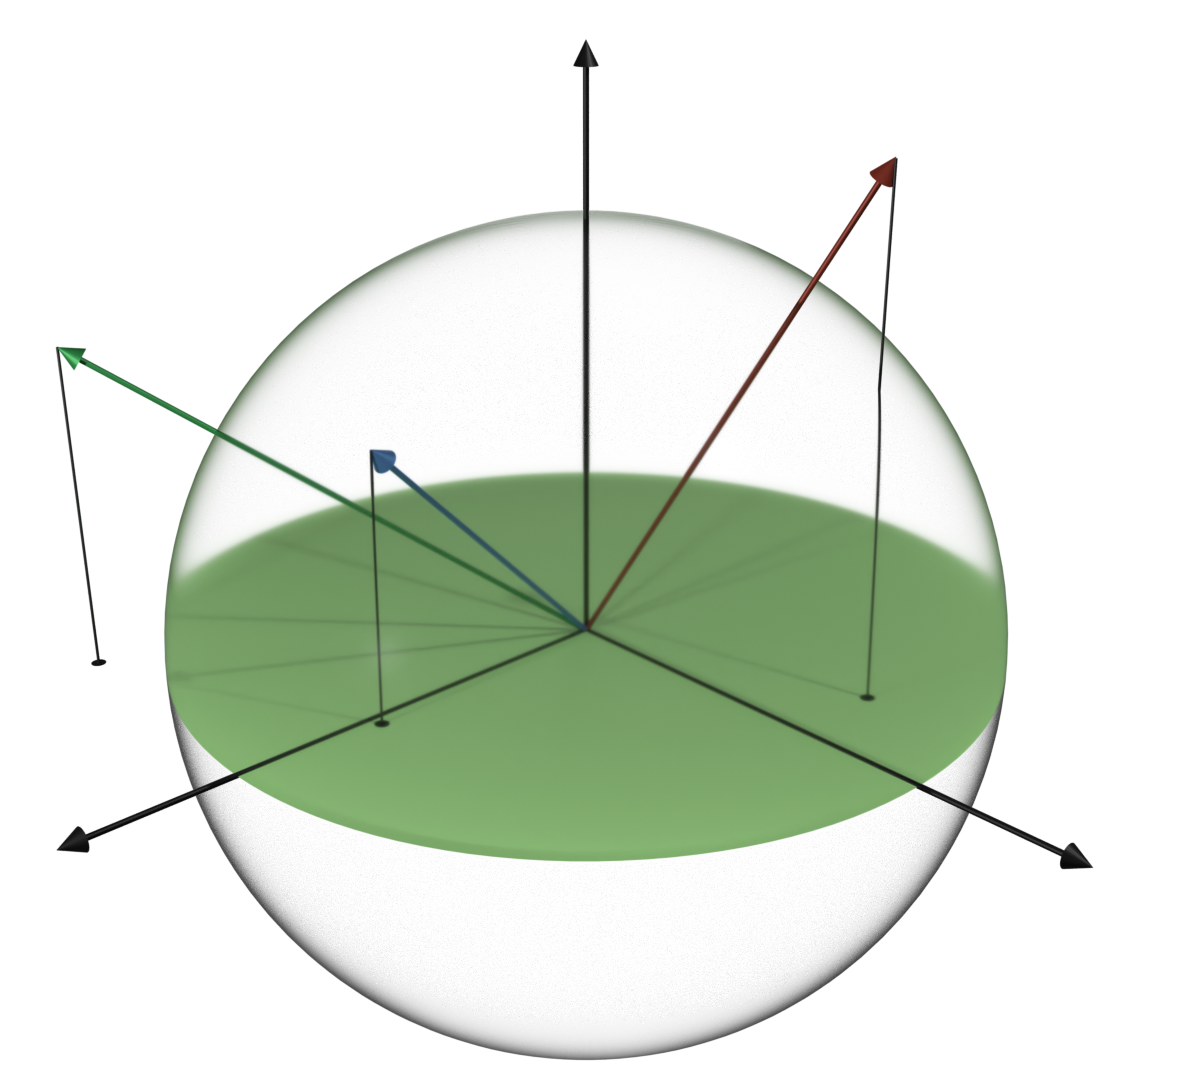
\includegraphics[width=0.75\textwidth]{figures/tiltSphere.png}
  % 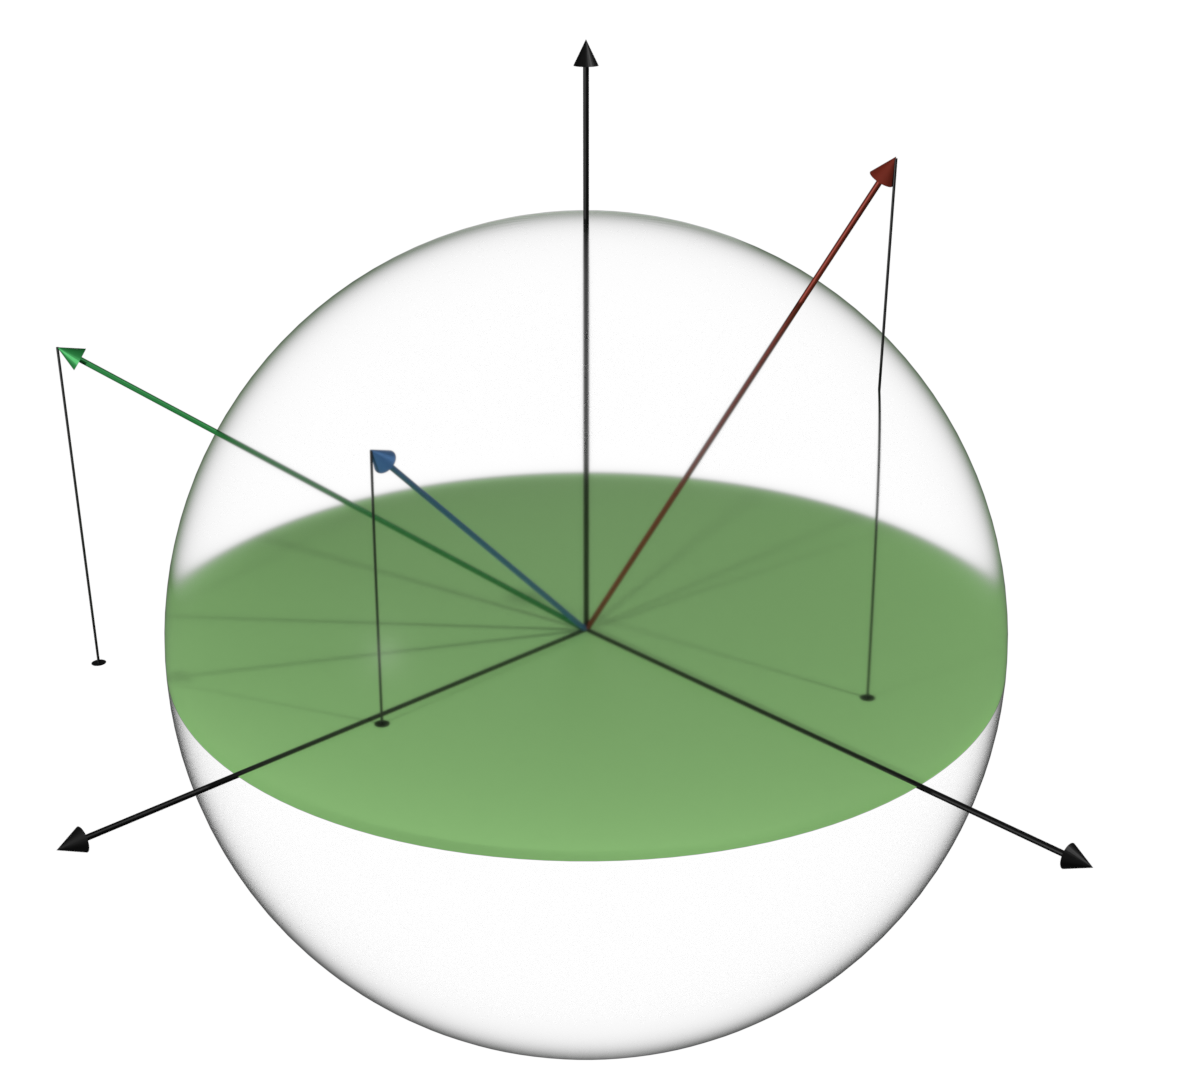
\includegraphics[width=0.75\textwidth]{figures/tiltSpherewactualWhiteBackground.png}
  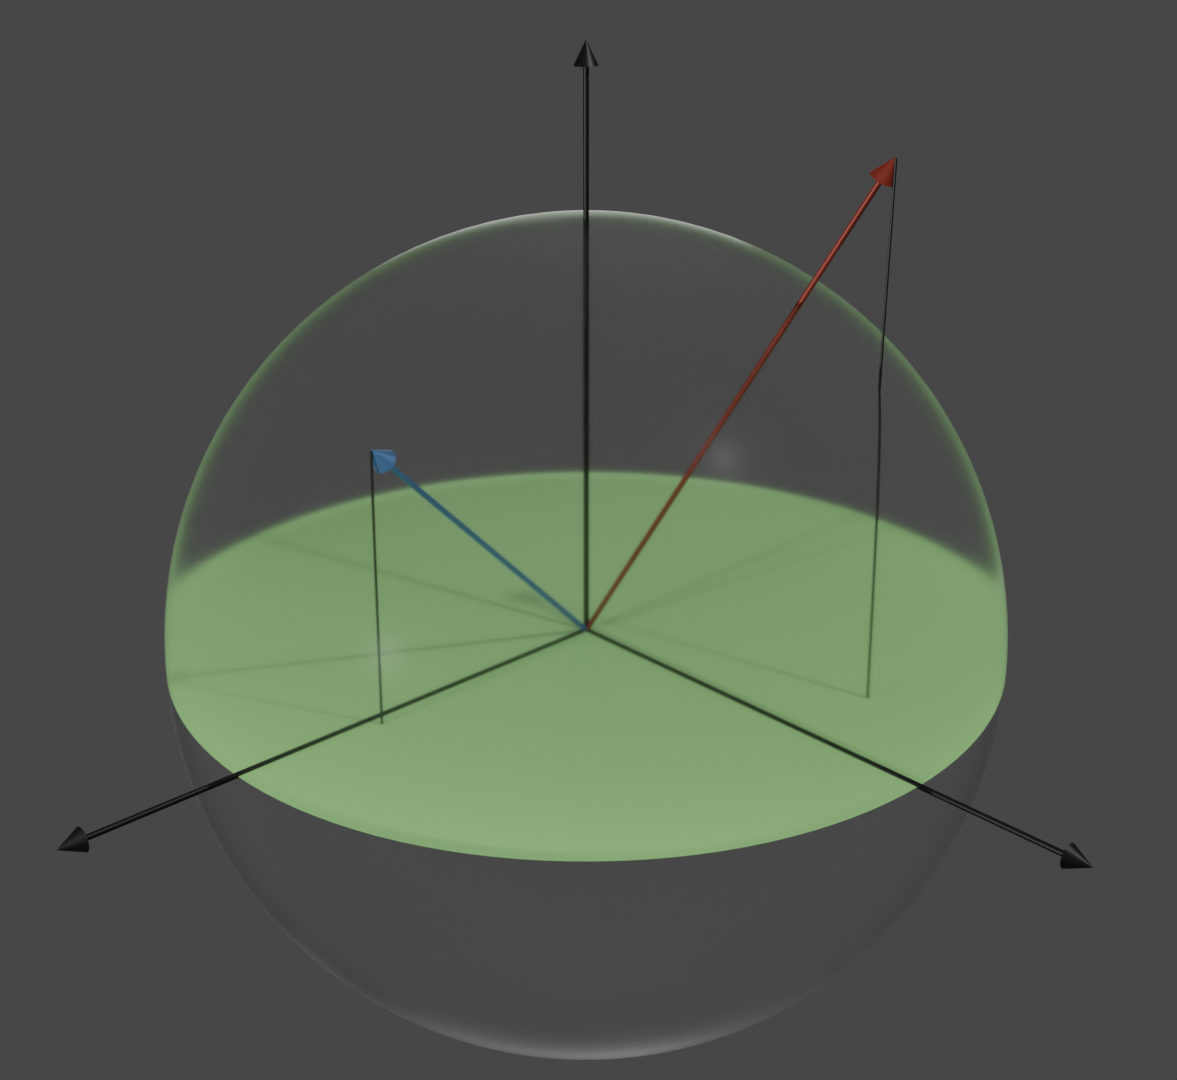
\includegraphics[width=0.75\textwidth]{figures/tiltSpherewBackground.png}
  \caption{Geometric visualization of the \emph{tilt vector} \( \vec{t} \).
    When the vector is inside the unit sphere (\( t < 1 \)), the system is in the Type-I regime.
    When the vector is outside the unit sphere (\( t > 1 \)), the system is in the Type-II regime.
    When the projection onto the \( xy \)-plane is on the unit disc, the system is in the \emph{magnetic} regime, otherwise it is in the \emph{electric} regime.
    Shown is Type-I tilt (blue), Type-II magnetic (red), and Type-II electric (green).
    Figure inspired by \textcite{tchoumakovMagneticFieldInducedRelativisticProperties2016}.
\label{fig:tiltSphere}
  }
\end{figure}

We now return to solving Eq.~\eqref{eq:32}, using the solution angle we just found.
By insertion, and after some clean up, we get
% \emph{note to thorvald: we chose \(\theta = Log \left(+ \dots\right) \)}
% \begin{multline}
%   \label{eq:39}
%   (R H_{B} R - E R^2 ) \ket{\tilde{\psi}} = 0
%   = v_F\\
%   \times \begin{pmatrix}
%           k_z ( s + t^s_z \gamma ) - E / v_F \gamma & -s ( ik_y + k_z t_x t_z \gamma - k_x / \gamma - E /v_{F} \gamma t^s_x)\\
%           s ( i k_y - k_z t_x t_z \gamma + k_x / \gamma + E /v_F \gamma t^s_x) & - k_z (s - t^s_z \gamma) - E /v_F \gamma
%         \end{pmatrix}
%     \ket{\tilde{\psi}}.
% \end{multline}
\begin{equation}
  \label{eq:39}
  (R H_{B} R - E R^2 ) \ket{\tilde{\psi}}
  = v_F  A \ket{\tilde{\psi}} = 0,
\end{equation}
with
\begin{align*}
  A_{11} &=   k_z ( s + t_{\parallel}^s \gamma ) - E / v_F \gamma,\\
  A_{12} &=  -s ( ik_y + k_z t_\perp t_\parallel \gamma - k_x / \gamma - E /v_{F} \gamma t_{\perp}^s),\\
  A_{21} &= s ( i k_y - k_z t_\perp t_\parallel \gamma + k_x / \gamma + E /v_F \gamma t_{\perp}^s),\\
  A_{22} &= - k_z (s - t_{\parallel}^s \gamma) - E /v_F \gamma.
\end{align*}
In order to simplify this further, absorb \(\gamma t_{\perp}^s (k_{z} t_{\parallel}^s - E /v_{F}) \) into \(k_{x}\).
Thus, let
\begin{equation}
  \label{eq:40}
  \begin{split}
    \tilde{k}_{x} &= k_{x} / \gamma + \gamma t_{\perp}^s ( E /v_F - k_{z} t_{\parallel}^s),\\
    \tilde{k}_{y} &=  k_{y},\\
    \tilde{k}_{z} &=  k_{z}.\\
  \end{split}
\end{equation}

These expressions warrant some explanation, as the Lorentz boost is of course
\begin{equation}
  \label{eq:41}
  \tilde{k}_x = \gamma (k_x - t_{\perp} \frac{E}{v_{F}}),
\end{equation}
where we used the four momentum \( p^{\mu } = (\frac{E}{v_{F}}, \vec{p}) \), and the effective speed of light \( v_F \).
It can thus look like our expression in Eq. \eqref{eq:40} is wrong.
The solution to this seeming inconsitency is that the proper energy is not \( \frac{E}{v_{F}} - k_z t_{\parallel} \), but rather \( \frac{E}{v_{F}} - k_z t_{\parallel} - k_x t_{\perp}\).
\todo{Something smart here, or remove discussion}

The eigenvalue equation is simply
\begin{equation}
  \label{eq:42}
  \left[  \gamma \left( t^s_{\parallel} \tilde{k}_{z} - \frac{E}{v_{F}} \right) \mathcal{I}_{2} +
  s \tilde{k}_{i} \sigma _{i} \right] \ket{\tilde{\psi}}= 0.
\end{equation}
If we now again introduce the magnetic field using minimal coupling, \(k_{x} \to  k_{x} - ey B_{z} \), this corresponds to an effective field \(B_{z} /\gamma \) in the new quantities.
This is because \(\tilde{k}_{x} \to  \tilde{k}_{x} - e y B_{z} /\gamma \).
The Landau level equation thus reads
\begin{equation}
  \label{eq:43}
  \left[
  \sum\limits_{i} s v_{F} \left(\tilde{k}_{i} + e \tilde{A}_{i} \right) \sigma _{i}
\right  ] \ket{\tilde{\psi}} =
(E- t^s_{\parallel} v_{F} \tilde{k}_{z}) \gamma \ket{\tilde{\psi}},
\end{equation}
where \(\vec{\tilde{A}}=-B_{z}/ \gamma y \hat{x}\).
We may thus use directly the result for the untilted cone, Eq.~\eqref{eq:26}, giving
\begin{subequations}
  \label{eq:44}
  \begin{align}
    \left(E - t^s_{\parallel} v_{F} \tilde{k}_{z} \right) \gamma &= \sign (m) v_{F} \sqrt{2 |m| e \frac{B}{ \gamma }  + \tilde{k}_{z}^2}, & m \neq 0,\\
    \left(E - t^s_{\parallel} v_{F} \tilde{k}_{z} \right) \gamma &= - s   \tilde{k}_{z} v_{F}, & m=0.
  \end{align}
\end{subequations}
Cleaning up, we get
\begin{subequations}
  \label{eq:45}
  \begin{align}
    E &= t^s_{\parallel} v_F \tilde{k}_{z} + \sign(m) v_F \sqrt{2 |m| e \frac{B}{\gamma ^3}  + \tilde{k}_{z}^2 /\gamma ^2}, & m\neq 0,\\
    E &= \tilde{k}_{z} v_{F} \left( t^s_{\parallel}  - s  / \gamma  \right), & m=0.
  \end{align}
\end{subequations}

As the perpendicular tilt is increased, \(\gamma = 1 / \sqrt{1-t_{\perp} ^{2}}\) diverges to infinity.
With the trivial substitution \(\alpha = 1 /\gamma \), which goes to zero, this gets an intuitive interpretation.
As the perpendicular tilt increases, the Landau levels converge towards \(t_{\parallel} v_{F} \tilde{k}_{z}\).
In particular, the separation between Landau levels is reduced by a factor \(\alpha ^{3 /2}\).
The effect of the tilt on the Landau levels is to squeeze the Landau levels together, and we will call the \(\alpha \) the \emph{squeezing factor}.
We note that when approaching the degree of tilt where we are no longer able to find a boost which enables us to solve for the Landau levels, i.e. when \( |t_{\perp}| \to 1\), the squeezing factor goes to zero.
As the tilt exceeds this limit, the squeezing factor is imaginary.
The Landau level description is only valid for \( |t_{\perp}| < 1 \).

The energy levels of the tilted cone expressed in terms of the energy levels of the untilted cone
\[
E = t^s_{\parallel} v_F k_z + \alpha E^0_{m, \alpha B},
\]
where \( E^0_{m, \alpha B} \) is the energy in the untilted case, with magnetic field \( \alpha B \).
Tilting of the Landau levels is induced by the parallel tilt component, \( t_\parallel \).
In fact, the Landau levels cross the Fermi level at the transition from Type-I to Type-II as well.
The Landau levels are shown in Figure~\ref{fig:llevelstilt}.


\begin{figure}[p!]
  \centering
  \resizebox{\textwidth}{!}{
  \newcommand{\LLplot}[2]{
  %% #1 is alpha, #2 is tz
  \addplot[forget plot]{(#2-#1) * x};  % Zeroth level
  \addplot[forget plot, black!60, dash pattern={on 3pt off 2pt on 1pt off 2pt on 1pt off 2pt on 1pt off 2pt}]{(-#2+#1) * x};  % Zeroth level, s=-1
  \addplot[forget plot, dashed]{(#2+#1) * x};  % Zeroth level, s=-1, P broken
  \addplot[forget plot, dotted]{(-#2-#1) * x};  % Zeroth level, s=1, tz<1
  \addplot[dashed, forget plot, gray] {0};
  \pgfplotsforeachungrouped \n in {1,...,5} {
    \addplot+[red, forget plot, solid] {#2 * x + #1 * sqrt(\n * #1 + x^2)};  % Positive E
    \addplot+[blue, solid] {#2 * x - #1 * sqrt(\n * #1 + x^2)};  % Negative E
  }
  \pgfplotsforeachungrouped \n in {1,...,5} {
    \addplot+[red, forget plot, dotted] {-#2 * x + #1 * sqrt(\n * #1 + x^2)};  % Positive E
    \addplot+[blue, dotted] {-#2 * x - #1 * sqrt(\n * #1 + x^2)};  % Negative E
  }
}

\tikzsetnextfilename{lllevels}
%% \hspace{-1.6cm}
\begin{tikzpicture}
  \begin{groupplot} [%
    % width=0.64\textwidth, %% Width of each window... Can be set more elegantly, but here just trial and error
    cycle list name=linestyles,
    samples=100,
    ymin=-2.5,ymax=2.5,
    xmin=-3.9, xmax=3.9,
    xlabel=\( \kappa_z \),
    ylabel=\( \epsilon_{\kappa_z m s} \),
    group style={
      x descriptions at=edge bottom,
      y descriptions at=edge left,
      horizontal sep=4pt, vertical sep=4pt,
      group size=2 by 3,
    },
    ]
    \newcommand\varalpha{1}
    \newcommand\vartz{0}
    %%
    \nextgroupplot
    \LLplot{\varalpha}{\vartz}
    \pgfmathsetmacro\hfirst{\vartz-\varalpha}
    \pgfmathsetmacro\hsecond{\vartz * 1 + \varalpha * sqrt(\varalpha + 1)}
    \draw[->] (axis cs:1,\hfirst)--(axis cs:1, \hsecond);
    %%
    \nextgroupplot
    \renewcommand\varalpha{0.6}
    \renewcommand\vartz{0}
    \LLplot{\varalpha}{\vartz}
    \pgfmathsetmacro\hfirst{\vartz-\varalpha}
    \pgfmathsetmacro\hsecond{\vartz * 1 + \varalpha * sqrt(\varalpha + 1)}
    \draw[->] (axis cs:1,\hfirst)--(axis cs:1, \hsecond);
    %%

    \nextgroupplot
    \renewcommand\varalpha{1}
    \renewcommand\vartz{0.5}
    \LLplot{\varalpha}{\vartz}
    \pgfmathsetmacro\hfirst{\vartz-\varalpha}
    \pgfmathsetmacro\hsecond{\vartz * 1 + \varalpha * sqrt(\varalpha + 1)}
    \draw[->] (axis cs:1,\hfirst)--(axis cs:1, \hsecond);
    %%
    \nextgroupplot
    \renewcommand\varalpha{0.6}
    \renewcommand\vartz{0.5}
    \LLplot{\varalpha}{\vartz}
    \pgfmathsetmacro\hfirst{\vartz-\varalpha}
    \pgfmathsetmacro\hsecond{\vartz * 1 + \varalpha * sqrt(\varalpha + 1)}
    \draw[->] (axis cs:1,\hfirst)--(axis cs:1, \hsecond);

    \pgfmathsetmacro\x{-0.8}
    \pgfmathsetmacro\gfirst{\vartz * \x - \varalpha * sqrt(1 * \varalpha + (\x)^2)}
    \pgfmathsetmacro\gsecond{\vartz * \x + \varalpha * sqrt(4 * \varalpha + (\x)^2)}
    \draw[brown, ->] (axis cs:\x,\gfirst)--(axis cs:\x, \gsecond);  %% Higher order transition
    %%
    \nextgroupplot
    \renewcommand\varalpha{1}
    \renewcommand\vartz{1.2}
    \pgfmathsetmacro\x{-sqrt(\varalpha^2/(\vartz^2-\varalpha^2))-0.3}
    \LLplot{\varalpha}{\vartz}
    \pgfmathsetmacro\hfirst{\vartz * \x + \varalpha * sqrt(\varalpha + (\x)^2)}
    \pgfmathsetmacro\hsecond{\vartz * \x + \varalpha * sqrt(2 * \varalpha + (\x)^2)}
    \draw[teal!80!black, ->, thick] (axis cs:\x,\hfirst)--(axis cs:\x, \hsecond);  %% Intraband
    %%
    \nextgroupplot
    \renewcommand\varalpha{0.6}
    \renewcommand\vartz{1.2}
    \pgfmathsetmacro\x{-sqrt(\varalpha^2/(\vartz^2-\varalpha^2))/2}
    \LLplot{\varalpha}{\vartz}
    \pgfmathsetmacro\hfirst{(\vartz - \varalpha) * \x}
    \pgfmathsetmacro\hsecond{\vartz * \x + \varalpha * sqrt(1 * \varalpha + (\x)^2)}
    \draw[->] (axis cs:\x,\hfirst)--(axis cs:\x,\hsecond);
  \end{groupplot}
\end{tikzpicture}

  }
  % \includegraphics[width=0.8\textwidth]{example-image-10x16}
  \caption{\label{fig:llevelstilt}Landau levels for different values of \( t_x, t_z \).
    The top two rows show Type-I, while the lowest row shows Type-II.
    Left column shows \( t_x = 0 \), right column \( t_x = 0.64 \) (\( \alpha = 0.6 \)).
    The rows shows \( t_z = 0, 0.5, 1.2 \), from top to bottom.
    The dotted lines show the Landau levels with opposite sign of \( t_z \), the dashed show the opposite chirality.
    The arrows indicate valid ``transitions'', namely the \( 0\to 1 \) interband in black, \( -1 \to 4 \) interband in \textcolor{brown!70!black}{brown}, and \( 1\to 2 \) intraband in \textcolor{teal!70!black}{teal}.
  }
\end{figure}

The eigenstate of
\[
H = v_{F} \sigma ^{i} ( p_{i} + e A_{i} ),
\]
with \(A_{i} = - B_{z} y \delta _{i x}\), given in the position basis, is
\begin{equation}
  \phi _{\vec{k} m s}(\vec{r}) = \frac{1}{\sqrt{L_xL_z}}
  \frac{e^{ik_x x}e^{ik_z z}}{\sqrt{\alpha_{k_z m s}^2 + 1}}
  e^{-\frac{y-k_x l^2}{2 l_B^2}}
  \begin{pmatrix}
    \frac{\alpha_{k_z m s}}{\sqrt{2^{M-1} (M-1)! \sqrt{\pi } l_B}} H_{M-1}\left( \frac{y-k_x l_B^2}{l_B} \right)\\
    \frac{1}{\sqrt{2^M M! \sqrt{\pi } l_B}} H_M \left( \frac{y-k_x l_B^2}{l_B} \right)
  \end{pmatrix},
\end{equation}
where capital letters indicate absolute value of corresponding quantity, $M=|m|, \vec{k} = (k_x, k_z)$, and with the normalization factor
\begin{equation}
  \alpha_{k_z m s} = \frac{-\sqrt{2eB M}}{\frac{E_{k_z m s}}{s v_{F}} -   k_z}.
\end{equation}
Taking care to keep track of boosted and rescaled quantites, the eigenstate in the boosted frame is
\begin{equation}
  \label{eq:47}
  \tilde{\psi}(\tilde{\vec{r}}) =
  \frac{1}{\sqrt{L_xL_z}}
  \frac{e^{i \tilde{k}_x \tilde{x}}e^{i k_z z}}{\sqrt{\alpha_{\tilde{k}_z m s}^2 + 1}}
  e^{-\frac{\left(\tilde{y} - \tilde{k}_x l_{B'}^2\right)^2}{2 l_{B'}^2}}
  \begin{pmatrix}
    \frac{\alpha_{\tilde{k}_z m s}}{\sqrt{2^{M-1} (M-1)! \sqrt{\pi } l_{B'}}} H_{M-1}\left( \frac{\tilde{y} - \tilde{k}_x l_{B'}^2}{l_{B'}} \right)\\
    \frac{1}{\sqrt{2^M M! \sqrt{\pi } l_{B'}}} H_M \left( \frac{\tilde{y} - \tilde{k}_x l_{B'}^2}{l_{B'}} \right)
  \end{pmatrix},
\end{equation}
with
\begin{equation}
  \alpha_{\tilde{k}_z m s} = \frac{-\sqrt{2e B'  M}}{ \gamma \frac{E_{\tilde{k}_z m s} - t^s_{\parallel} v_{F} \tilde{k}_{z}}{s v_{F}} -   \tilde{k}_z},
\end{equation}
where
\[
B' = B \alpha.
\]
We note that \( \alpha_{k_z 0 s} = 0 \), so using the explicit form of the energy we may simplify the expression some.
For \( m\neq 0 \)
\[
  \frac{
    E_{k_z m s} - t^s_{\parallel} v_F k_z
  }{s v_{F}} = \sign(m) s \alpha \sqrt{2 M e B \alpha + k_{z}^2}
\]
and thus
\begin{equation}
  \label{eq:48}
  \alpha_{k_z m s} =
  \frac{-\sqrt{ \alpha M }}{\sign(m) s \sqrt{\alpha M + \kappa^2} - \kappa}
\end{equation}
where we defined the dimensionless \( \kappa_z = \sqrt{2 e B} k_z  \).

The original eigenstate \(\ket{\psi } = 1 /\mathcal{N} e^{\theta /2 \sigma _{x}} \ket{\tilde{\psi} }\) of the tilted system is easily found.
Reinserting explicitly, in the boosted frame, that
\[
  \tilde{k}_{x} = \alpha k_{x} + \frac{t_{\perp}^s}{\alpha} (E_{k_z m s} /v_F- k_{z} t_{\parallel}^s)
  = \alpha k_x + t_{\perp}^s \frac{E^0_{m, \alpha B} }{v_{F}}
\]
and \(l_{B'}=\frac{l_{B}}{\sqrt{\alpha} }\)
we define
\begin{equation}
  \label{eq:49}
  \chi =
  \frac{y-\tilde{k}_{x} l_{B'}^2}{l_{B'}}
  =
  \sqrt{\alpha } (y-k_{x} l_{B}^2) /l_{B}
  + \frac{ t_{\perp}^s l_B }{ \sqrt{\alpha} v_F} E^{0}_{m, \alpha B},
\end{equation}
which is the argument of the Hermite polynomials.
For later convenience, let us explicitly define
\begin{equation}
  \label{eq:50}
  \tilde{\phi} _{\vec{k} m s} (\vec{\tilde{r}}) =
  \frac{e^{i \tilde{k}_{x} \tilde{x} + i k_{z} z}}{\sqrt{L_{x} L_{z}} }
  \underbrace{
  \frac{
    e^{-\frac{1}{2} \chi ^2}
    \sqrt[4]{\alpha }
  }
  {\sqrt{\alpha^2_{\tilde{k}_{z} m s} + 1} }
  \begin{pmatrix}
    \frac{\alpha_{\tilde{k}_z m s}}{\sqrt{2^{M-1} (M-1)! \sqrt{\pi } l_{B}}} H_{M-1}\left( \chi  \right)\\
    \frac{1}{\sqrt{2^M M! \sqrt{\pi } l_{B}}} H_M \left( \chi \right)
  \end{pmatrix}}_{\tilde{\phi}_{\vec{k} m s} (y)},
\end{equation}
and thus
\begin{equation}
  \label{eq:51}
  \tilde{\phi}_{\vec{k} m s} (y) =
  e^{-\frac{1}{2} \chi ^2}
  \begin{pmatrix}
    a_{\vec{k} m s} H_{M-1} (\chi)\\
    b_{\vec{k} m s} H_{M} (\chi)
  \end{pmatrix},
\end{equation}
with
\begin{align}
 \label{eq:52}
  a_{\vec{k} m s} &=
                    \frac{
                    \alpha_{\tilde{k}_z m s} \sqrt[4]{\alpha }
                    }{
                    \sqrt{\alpha^2 _{\tilde{k}_z m s} + 1}
                    \sqrt{2^{M-1} (M-1)! \sqrt{\pi} l_B}
                    },\\
  \label{eq:53}
  b_{\vec{k} m s} &=
                    \frac{
                     \sqrt[4]{\alpha }
                    }{
                    \sqrt{\alpha^2 _{\tilde{k}_z m s} + 1}
                    \sqrt{2^{M} M! \sqrt{\pi} l_B}
                    }.
\end{align}

We proceed now to find the normalization factor \( \mathcal{N} \), as it will become necessary in later steps.
Recall that
\[
  \ket{\psi} = \frac{1}{\mathcal{N}} e^{\theta /2 \sigma _x} \ket{\tilde{\psi}},
\]
and
\[
e^{\theta \sigma _x} =
\frac{1}{\alpha }
\begin{pmatrix}
  1 & -s t_{\perp}^s\\
  -s t_{\perp}^s & 1
\end{pmatrix}.
\]
The upper and lower part of the spinor are orthogonal, thus we have
\begin{equation}
  \label{eq:54}
  \braket{\psi  | \psi } = \frac{1}{\mathcal{N}^{*} \mathcal{N}} \frac{1}{\alpha } \braket{\tilde{\psi}  | \tilde{\psi} } = 1 \implies \mathcal{N}^{*}\mathcal{N} = \frac{1}{\alpha }.
\end{equation}
We choose \( \mathcal{N} = \alpha^{-\frac{1}{2}} \).

\begin{summary}\label{summary:llevels}
The tilted Hamiltonian
  \[
    H = v_F \vec{t}^s \vec{p} + s v_F \vec{p} \vec{\sigma}
  \]
  in a magnetic field \( \vec{B} \) has the Landau levels
  \[
    E =
    \begin{cases}
      t^s_{\parallel} v_F k_z + \sign(m) v_F \alpha \sqrt{2 e B \alpha M + k_{z} ^2} & m \neq 0,\\
      t^s_{\parallel} v_F k_z - s \alpha v_F k_z & m = 0,
    \end{cases}
  \]
  with the the \emph{squeezing factor} \( \alpha = \sqrt{1 - t_{\perp} ^2}  \).
  The associated eigenstates in the position basis are
  \[
    \psi(\vec{r}) = \sqrt{\alpha} e^{\theta /2 \sigma_x}
    \frac{
      e^{ik_{x} x + ik_{z} z}
    }{
      \sqrt{L_{x}  L_z}
    } \tilde{\psi}(y),
    \]
    where
    \[
      \tilde{\psi} (y) = e^{-\frac{1}{2} \chi^2}
      \begin{pmatrix}
        a_{k_z m s} H_{M - 1} (\chi) \\
        b_{k_z m s} H_M (\chi)
      \end{pmatrix},
    \]
    where we have defined \( \chi = \sqrt{\alpha} \frac{ y - k_x l_B^2 }{l_{B}} + \frac{t_{\perp}^s l_B}{\sqrt{\alpha} v_{F}} E^0_{m, \alpha B} \) and \( a_{k_z m s}, b_{k_z m s} \) are given in Eqs.~(\ref{eq:52}, \ref{eq:53}).
\end{summary}
